\chapter{Estado del Arte en Calificación Crediticia}

La calificación crediticia se obtiene mediante un conjunto de modelos de decisión que ayudan a los prestamistas a otorgar créditos. Estas técnicas son usadas para decidir quién obtiene crédito, cuánto crédito deben obtener, a qué precio lo tendrán, y qué estrategias operacionales mejorarán la rentabilidad de los clientes. Un puntaje de crédito puede ser transformado en la probabilidad del cliente de no pagar el préstamo. Así, desde el año 2000, se ha convertido en un pilar de los modelos desarrollados por instituciones financieras cumplir los requerimientos del Acuerdo de Basilea que dictamina que se deben estimar las probabilidades de morosidad de cada portafolio de préstamos \citep[1]{thomas2017credit}.

Con los avances en minería de datos y Big Data, ahora hay calificaciones crediticias siendo desarrolladas usando fuentes alternativas de datos. Estas pueden ser psicométricas, datos ``sociales'' en línea, o datos del teléfono móvil. Sin embargo, a parte de la consideración de por qué esta información debería ser predictiva del comportamiento crediticio, hay una mayor incertidumbre respecto al hecho de quiénes realmente poseen este tipo de información \citep[18]{thomas2017credit}.

Algunos desafíos claramente identificados en la creación de calificaciones crediticias están relacionados con la disponibilidad de los datos, su exactitud y su confiabilidad \citep[18--19]{thomas2017credit}. Sin embargo no trataremos estos temas porque están fuera del ámbito de esta investigación.

Cuando los puntajes de crédito se desarrollaron por primera vez en los años 1950s y 1960s, los únicos métodos utilizados fueron de discriminación estadística. Aún hoy, con el advenimiento de muchos nuevos enfoques de clasificación basados en minería de datos, los métodos estadísticos, especialmente la regresión logística son por mucho los métodos más utilizados para construir calificaciones crediticias \citep[25]{thomas2017credit}. Tienen la ventaja de permitir el uso de herramientas como los intervalos de confianza y prueba de hipótesis en el contexto de calificación crediticia. Así, uno es capaz de entender intuitivamente el funcionamiento del modelo construido y la importancia relativa de la diferentes características (variables) que constituyen el modelo. De esta forma, uno es capaz de usar esta información para proponer cambios en las preguntas hechas a los prestatarios.

Actualmente numerosas técnicas de clasificación han sido adoptadas para hacer calificación crediticia. Estas técnicas incluyen métodos estadísticos (e.g. análisis discrimante y regresión logística), modelos estadísticos no paramétricos (e.g. K-nearest neighbour y árboles de decisión) y redes neuronales. Con frecuencia surgen conflictos cuando se comparan las conclusiones de algunos de estos estudios. Por ejemplo, en \citep{desai1996comparison} encontraron que las redes neuronales se desempeñan considerablemente mejor que el análisis discriminante al predecir los malos préstamos, mientras que \citep{yobas2000credit} reportó que el segundo supera al primero. Por esto, el problema de escoger una técnica de clasificación para hacer la calificación crediticia permanece como una problema difícil y desafiante \citep{baesens2003benchmarking}.

Los últimos estudios comparativos en esta área son del año 2003 \citep{baesens2003benchmarking} y 2015 \citep{lessmann2015benchmarking}. En el último estudio comparativo de 2015 se compararon 41 métodos de clasificación a través de 8 conjuntos de datos. Además se creó una tabla muy interesante \citep{lessmann2015benchmarking} comparando los algoritmos de clasificación y evaluación utilizados en los últimos estudios. En dicha tabla se evidencia que los algoritmos más utilizados son las \ac{MLP}, las \ac{SVM} y métodos de ensamble. También se ve que los algoritmos de evaluación más utilizados son el \ac{AUC} y aquellos que involucran un umbral, como error de clasificación, \ac{TPR}, etc. También se incluye información sobre qué estudios utilizaron una validación estadística de la hipótesis.

A pesar de tener mucha investigación, la literatura sobre calificación crediticia no refleja varios recientes avances en aprendizaje predictivo \citep{lessmann2015benchmarking}. Estos avances conciernen 3 dimensiones:

\begin{itemize}
	\item Nuevos algoritmos de clasificación
	\item Nuevas medidas de desempeño para \textit{evaluar} modelos
	\item Pruebas de hipótesis estadísticas para \textit{comparar} modelos
\end{itemize}

Un análisis de le literatura de modelamiento de morosidad confirma que los estudios en esta área tienen varias limitaciones \citep{lessmann2015benchmarking}:

\begin{itemize}
	\item Utilizan pocos o pequeños conjuntos de datos
	\item No comparan diferentes clasificadores de estado del arte entre ellos
	\item Usan un pequeño conjunto de indicadores de exactitud conceptualmente similares
\end{itemize}

A continuación se dará un breve repaso de los algoritmos que se utilizarán en esta investigación, tanto para la clasificación como para la evaluación de los modelos.

\section{Algoritmos de clasificación base}
%En random forest hay que poner la diferencia con decision tree. %https://towardsdatascience.com/the-random-forest-algorithm-d457d499ffcd

\subsection{Regresión Logística}

Es un modelo estadístico que, en su forma básica, utiliza una regresión lineal transformada por una función logística para modelar una variable binaria dependiente. A continuación la definición formal.

Dado que $y\in \{0, 1\}$ es la clase real y $\vec{x}$ es el vector de características de entrada, donde $\vec{x}_0 = 1$ para tener un intercepto. La probabilidad de que $y=1$, dado $\vec{x}$, parametrizado por un vector de pesos $\vec{w}$,
se define en la fórmula \ref{eq:lr}.

\begin{equation}
	\label{eq:lr}
\begin{split}
	g(z) &= \frac{1}{1 + \exp(-z) } \\
	h &= P(y=1|\vec{x};\vec{w}) = g(\vec{w}\cdot\vec{x})
\end{split}
\end{equation}

A esta probabilidad se le conoce como hipótesis. En base a esta hipótesis, se define una función de costo en la fórmula \ref{eq:lr-loss} que penaliza cuando $y \ne h$.

\begin{equation}
	\label{eq:lr-loss}
\begin{split}
	C(h, y) &= -y \cdot \log{h} - (1-y) \log{h}
\end{split}
\end{equation}

Luego la función de costo del modelo de la fórmula \ref{eq:lr-loss-model}, es el promedio de la función de costo de todas las instancias del conjunto de entrenamiento.

\begin{equation}
	\label{eq:lr-loss-model}
\begin{split}
	J &= \frac{1}{m} \cdot \sum_{i=1}^{m} {C(h_i, y_i)}
\end{split}
\end{equation}

Esta función de costo del modelo es usada en el algoritmo de la gradiente descendente para ajustar los pesos $\vec{w}$ del modelo y de esta manera entrenarlo.

\subsection{Multi Layer Perceptron}

El modelo de Multi Layer Perceptron es la red neuronal más utilizada. Está inspirada por el funcionamiento del cerebro humano. Típicamente, se compone de tres capas, una capa de entrada, una capa de neuronas ocultas y una capa de salida. Cada neurona procesa su entrada y genera una salida que es transmitida a las neuronas en la siguiente capa.

\begin{figure}[htbp]
	\centering
	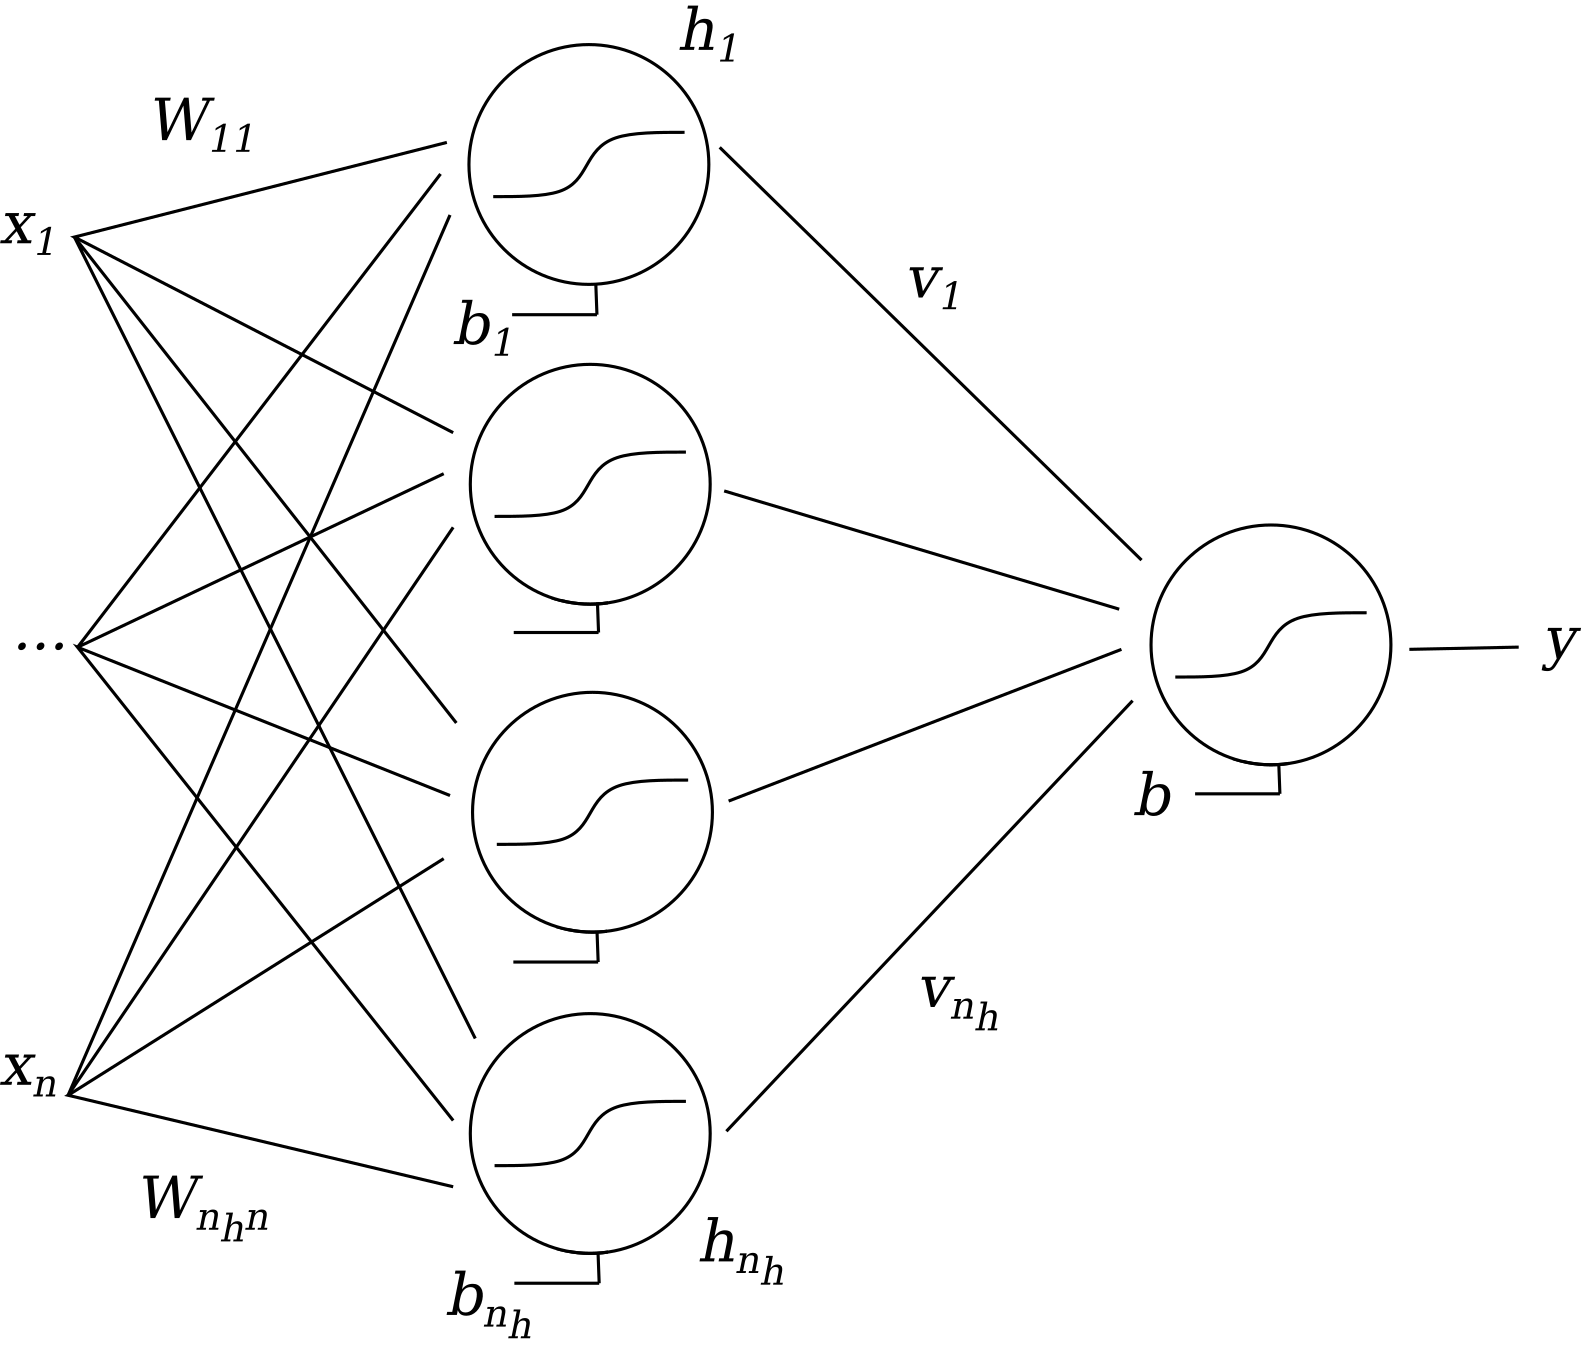
\includegraphics[width=0.6\linewidth]{graficos/propios/mlp.png}
	\caption{Arquitectura de una MLP típica \citep{bouzgou2012advanced}}
	\label{fig:mlp-eg}
\end{figure}

Tomando como ejemplo la figura \ref{fig:mlp-eg}, la salida de la neurona oculta $j$ es calculada procesando las entradas multiplicadas por sus respectivos pesos $w_{ij}$ y sumándole un bias $b_j$. Luego a este resultado le aplicamos una función de activación (ver fórmula \ref{eq:mlp-out}) que le permite a la red modelar relaciones no lineales en los datos. Esta función de activación suele ser la función logistica, la tangente hiperbólica o la función \ac{ReLU}. Para una comparación entre estas funciones ver figura \ref{fig:mlp-activation}

\begin{equation}
	\label{eq:mlp-out}
	h_j = f(b_j + \sum_{j=1}^{n_h} W_{ij} x_i)
\end{equation}

\begin{figure}[htbp]
	\centering
	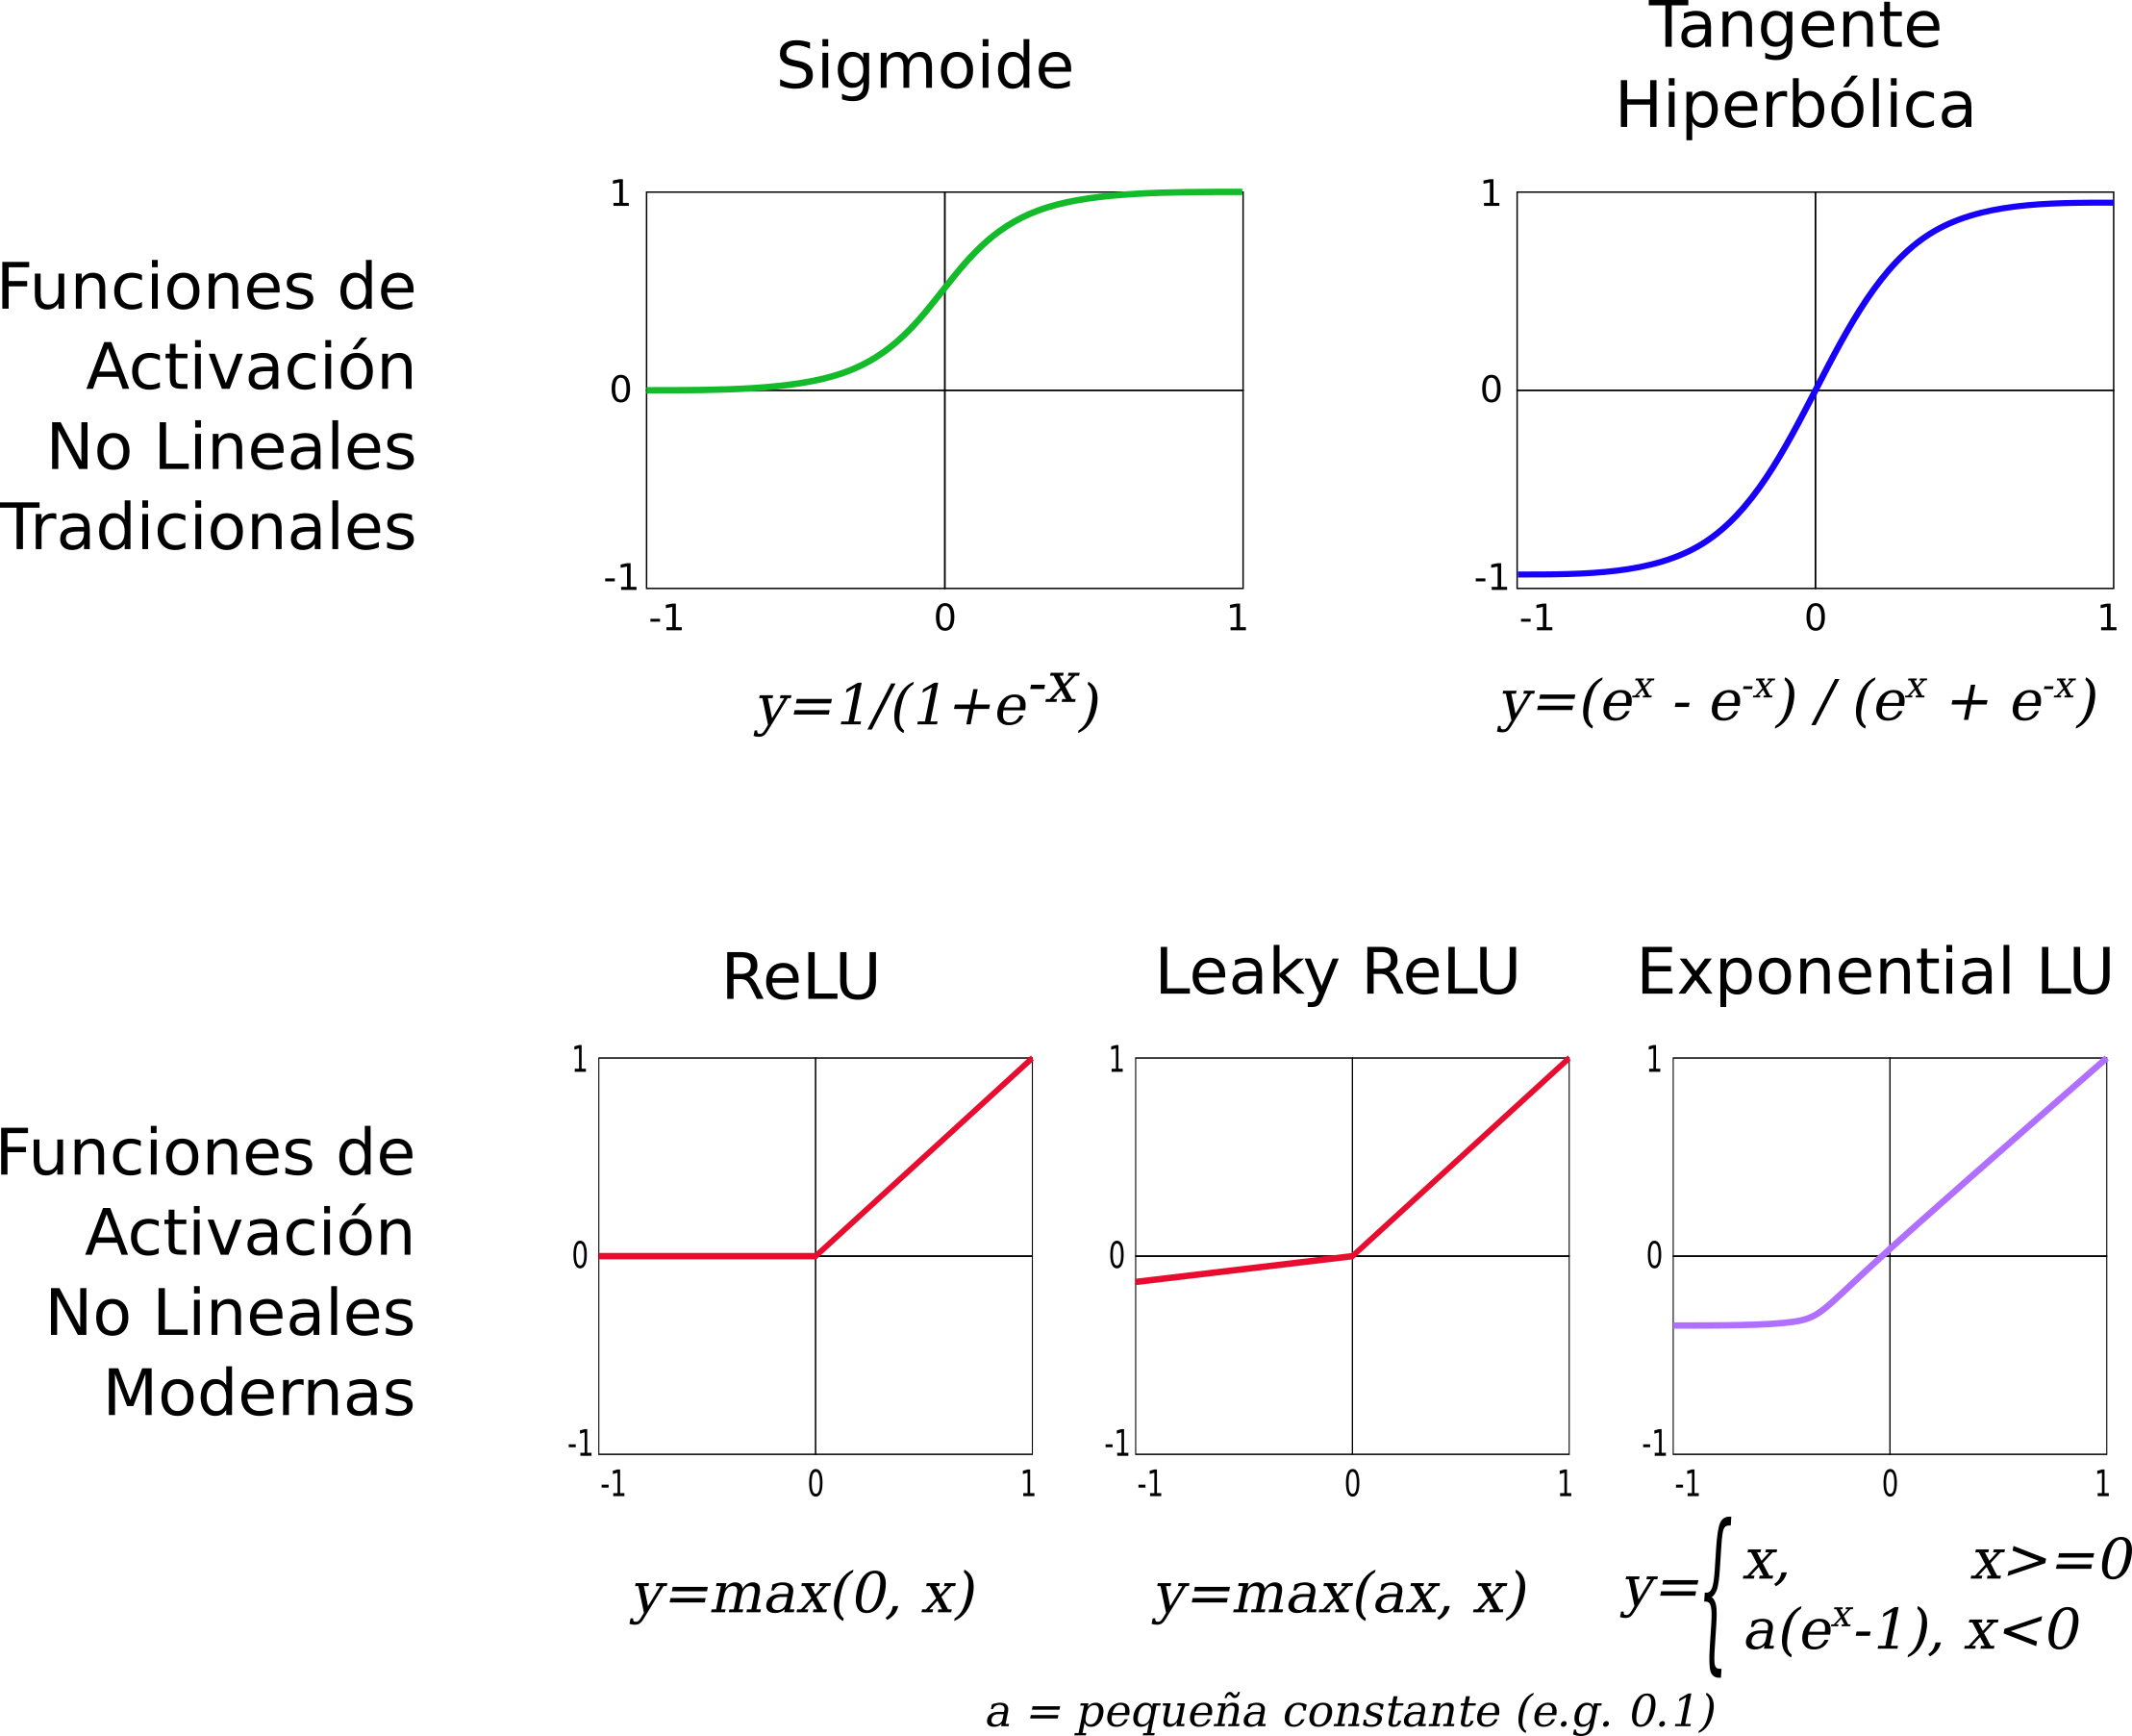
\includegraphics[width=0.8\linewidth]{graficos/propios/funciones_de_activacion.png}
	\caption{Funciones de activación \citep{sze2017efficient}}
	\label{fig:mlp-activation}
\end{figure}

\subsection{Deep Belief Network}

Es un tipo de red neuronal profunda, compuesta por múltiples capas de variables latentes (unidades ocultas), con conexiones entre las capas pero no entre unidades dentro de una misma capa.

El entrenamiento de esta red consiste en una etapa no supervisada seguida de otra supervisada. En la etapa no supervisada la \ac{DBN} aprende a reconstruir probabilísticamente sus entradas. Luego, se mejora la clasificación mediante la siguiente etapa de entrenamiento supervisado.

Las \ac{DBN} pueden ser vistas como la composición de redes simples no supervisadas tales como la \ac{RBM} o los autoencoders, donde la capa oculta de cada sub-red se convierte en la capa visible de la siguiente sub-red. Esta composición permite un proceso de entrenamiento no supervisado rápido capa por capa. Ver figura \ref{fig:dbn-train}.

\begin{figure}[htbp]
	\centering
	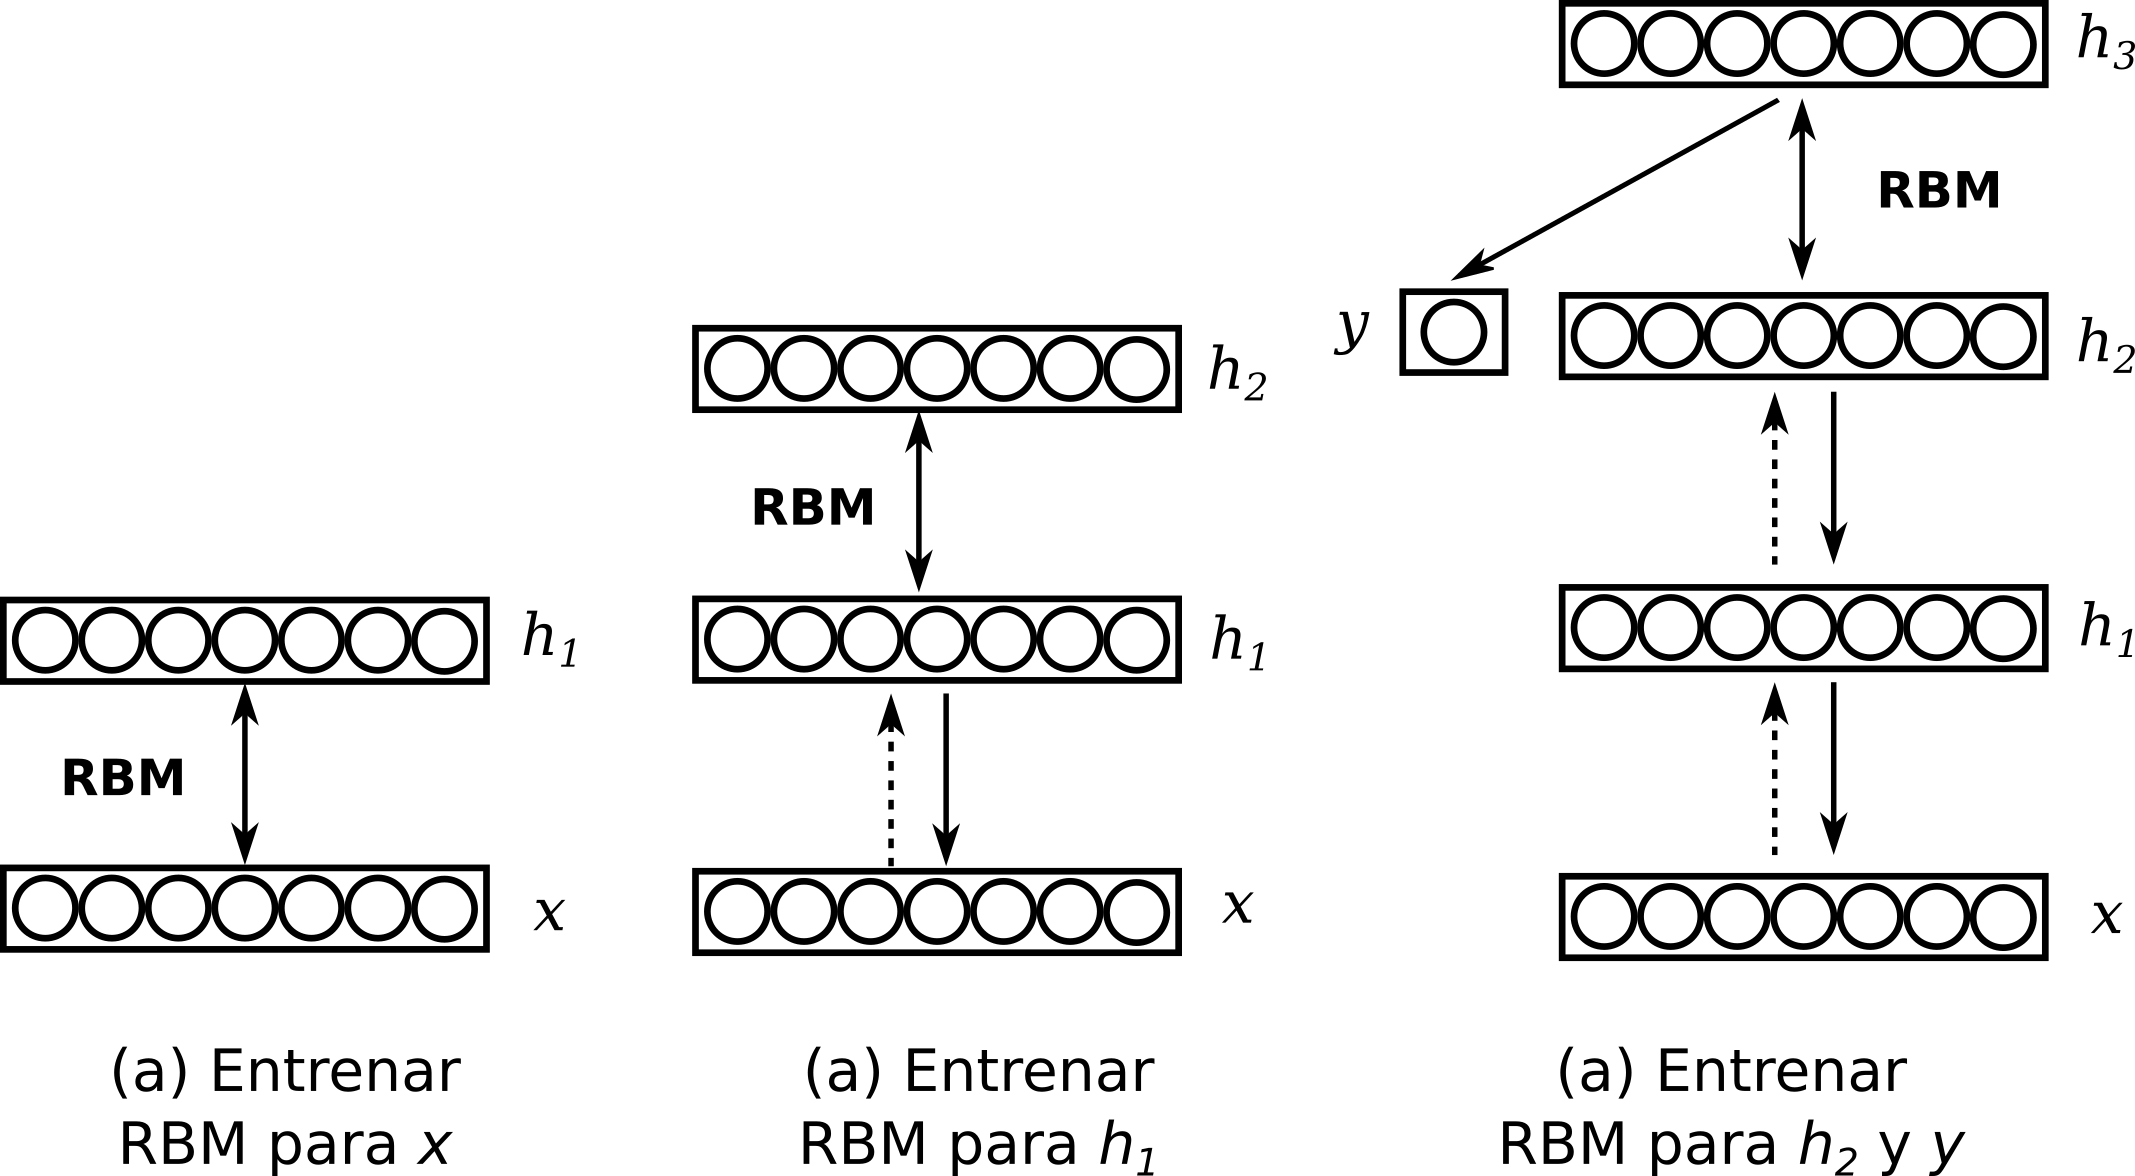
\includegraphics[width=0.9\linewidth]{graficos/propios/entrenamiento_dbn.png}
	\caption{Entrenamiento no supervisado de una DBN \citep{beysolow2017autoencoders}}
	\label{fig:dbn-train}
\end{figure}

\subsection{Support Vector Machine}

Es una familia de algoritmos de aprendizaje supervisado que pueden hacer clasificación y regresión \citep{cortes1995support}.

Funcionan construyendo un hiperplano o conjunto de hiperplanos en un espacio de dimensionalidad muy alta. Cada uno de estos hiperplanos está definido por el vector entre los dos puntos más cercanos de 2 clases diferentes, al que se llama vector de soporte. De esta manera se consigue separar a las clases con un margen máximo. La figura \ref{fig:svm-hiperplanos} ilustra esta forma de separación.

\begin{figure}[htbp]
	\centering
	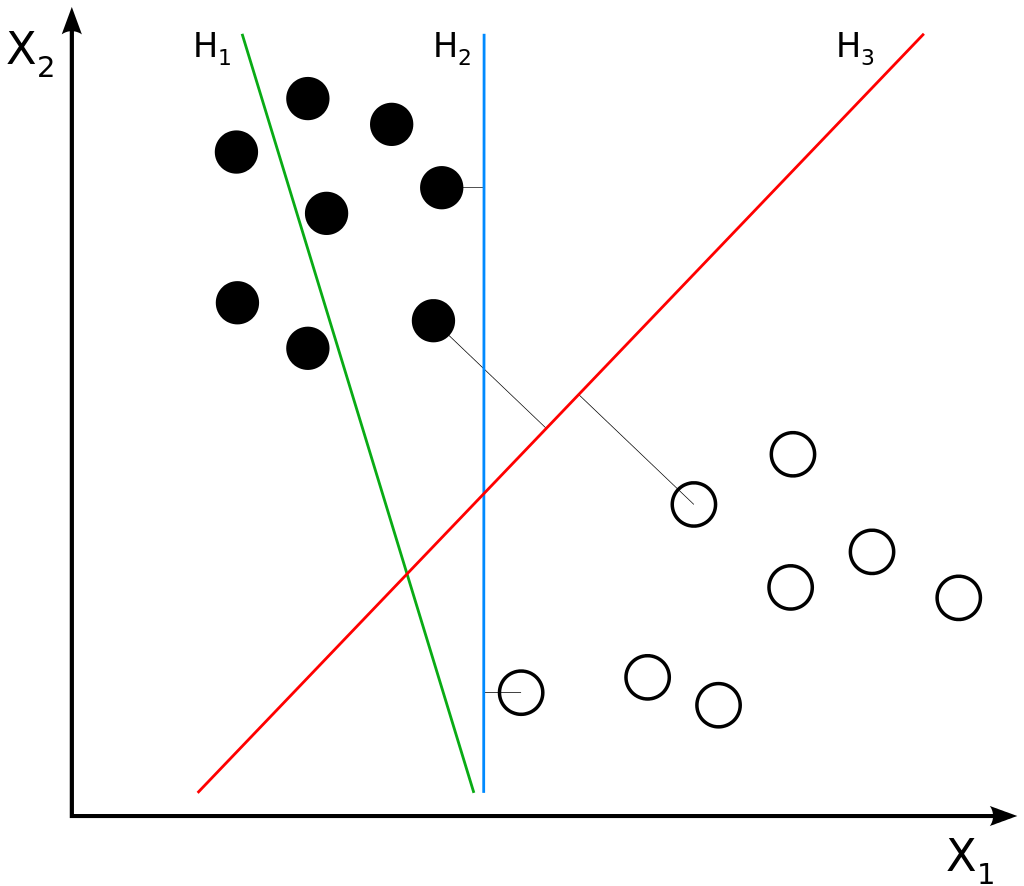
\includegraphics[width=0.4\linewidth]{graficos/svm_hiperplanos.png}
	\caption{Hiperplanos creados por una SVM \citep{wiki:svm_figure}}
	\label{fig:svm-hiperplanos}
	\par
	\small
	$H_1$ no separa las clases. $H_2$ las separa, pero solo con un margen pequeño. $H_3$ las separa con el margen máximo.
\end{figure}

Lamentablemente en las aplicaciones reales, las clases no suelen ser linealmente separables. Por eso existen las representaciones por medio de funciones de Kernel, que mapean el espacio de entradas $X$ a un espacio de características de mayor dimensionalidad, donde aumenta la capacidad computacional de las máquinas de aprendizaje lineal. Algunos tipos de función de Kernel son el Kernel Polinomial Homogéneo, el Kernel Perceptrón, la función de Base Radial Gaussiana y el Kernel Sigmoide \citep{cristianini2000introduction}.

Finalmente existe una versión de \ac{SVM} llamada \ac{LS-SVM}, que encuentra la solución resolviendo un conjunto de ecuaciones lineales en lugar de un problema convexo de programación cuadrática \citep{ak2002least}.

\subsection{Árbol de decisión}

Un árbol de decisión es un modelo simple de clasificación, se puede ver un ejemplo en la figura \ref{fig:dt-eg}. Cada nodo interno corresponde a una de las variables de entrada, y según el valor de esta se puede bajar a alguno de los nodos hijos. Cada hoja representa la predicción dada por los valores de la entrada representados por el camino desde la raíz hasta la hoja.

Los algoritmos para la construcción de árboles suelen trabajar de arriba hacia abajo, escogiendo una variable en cada paso que separa mejor los datos. Diferentes algoritmos usan diferentes métricas para definir una ``mejor separación de los datos''. Estos típicamente miden la homogeneidad de la variable objetivo en los subsets resultantes. Entre estos algoritmos tenemos la Impureza de Gini, la Ganancia de Información y la Reducción de la Varianza.

Entre las ventajas de los árboles de decisión tenemos que son fáciles de interpretar y requieren poca preparación de los datos. Sin embargo también tiene desventajas, como la tendencia al sobreajuste y la dificultad para aprender relaciones tipo XOR.

\begin{figure}[htbp]
	\centering
	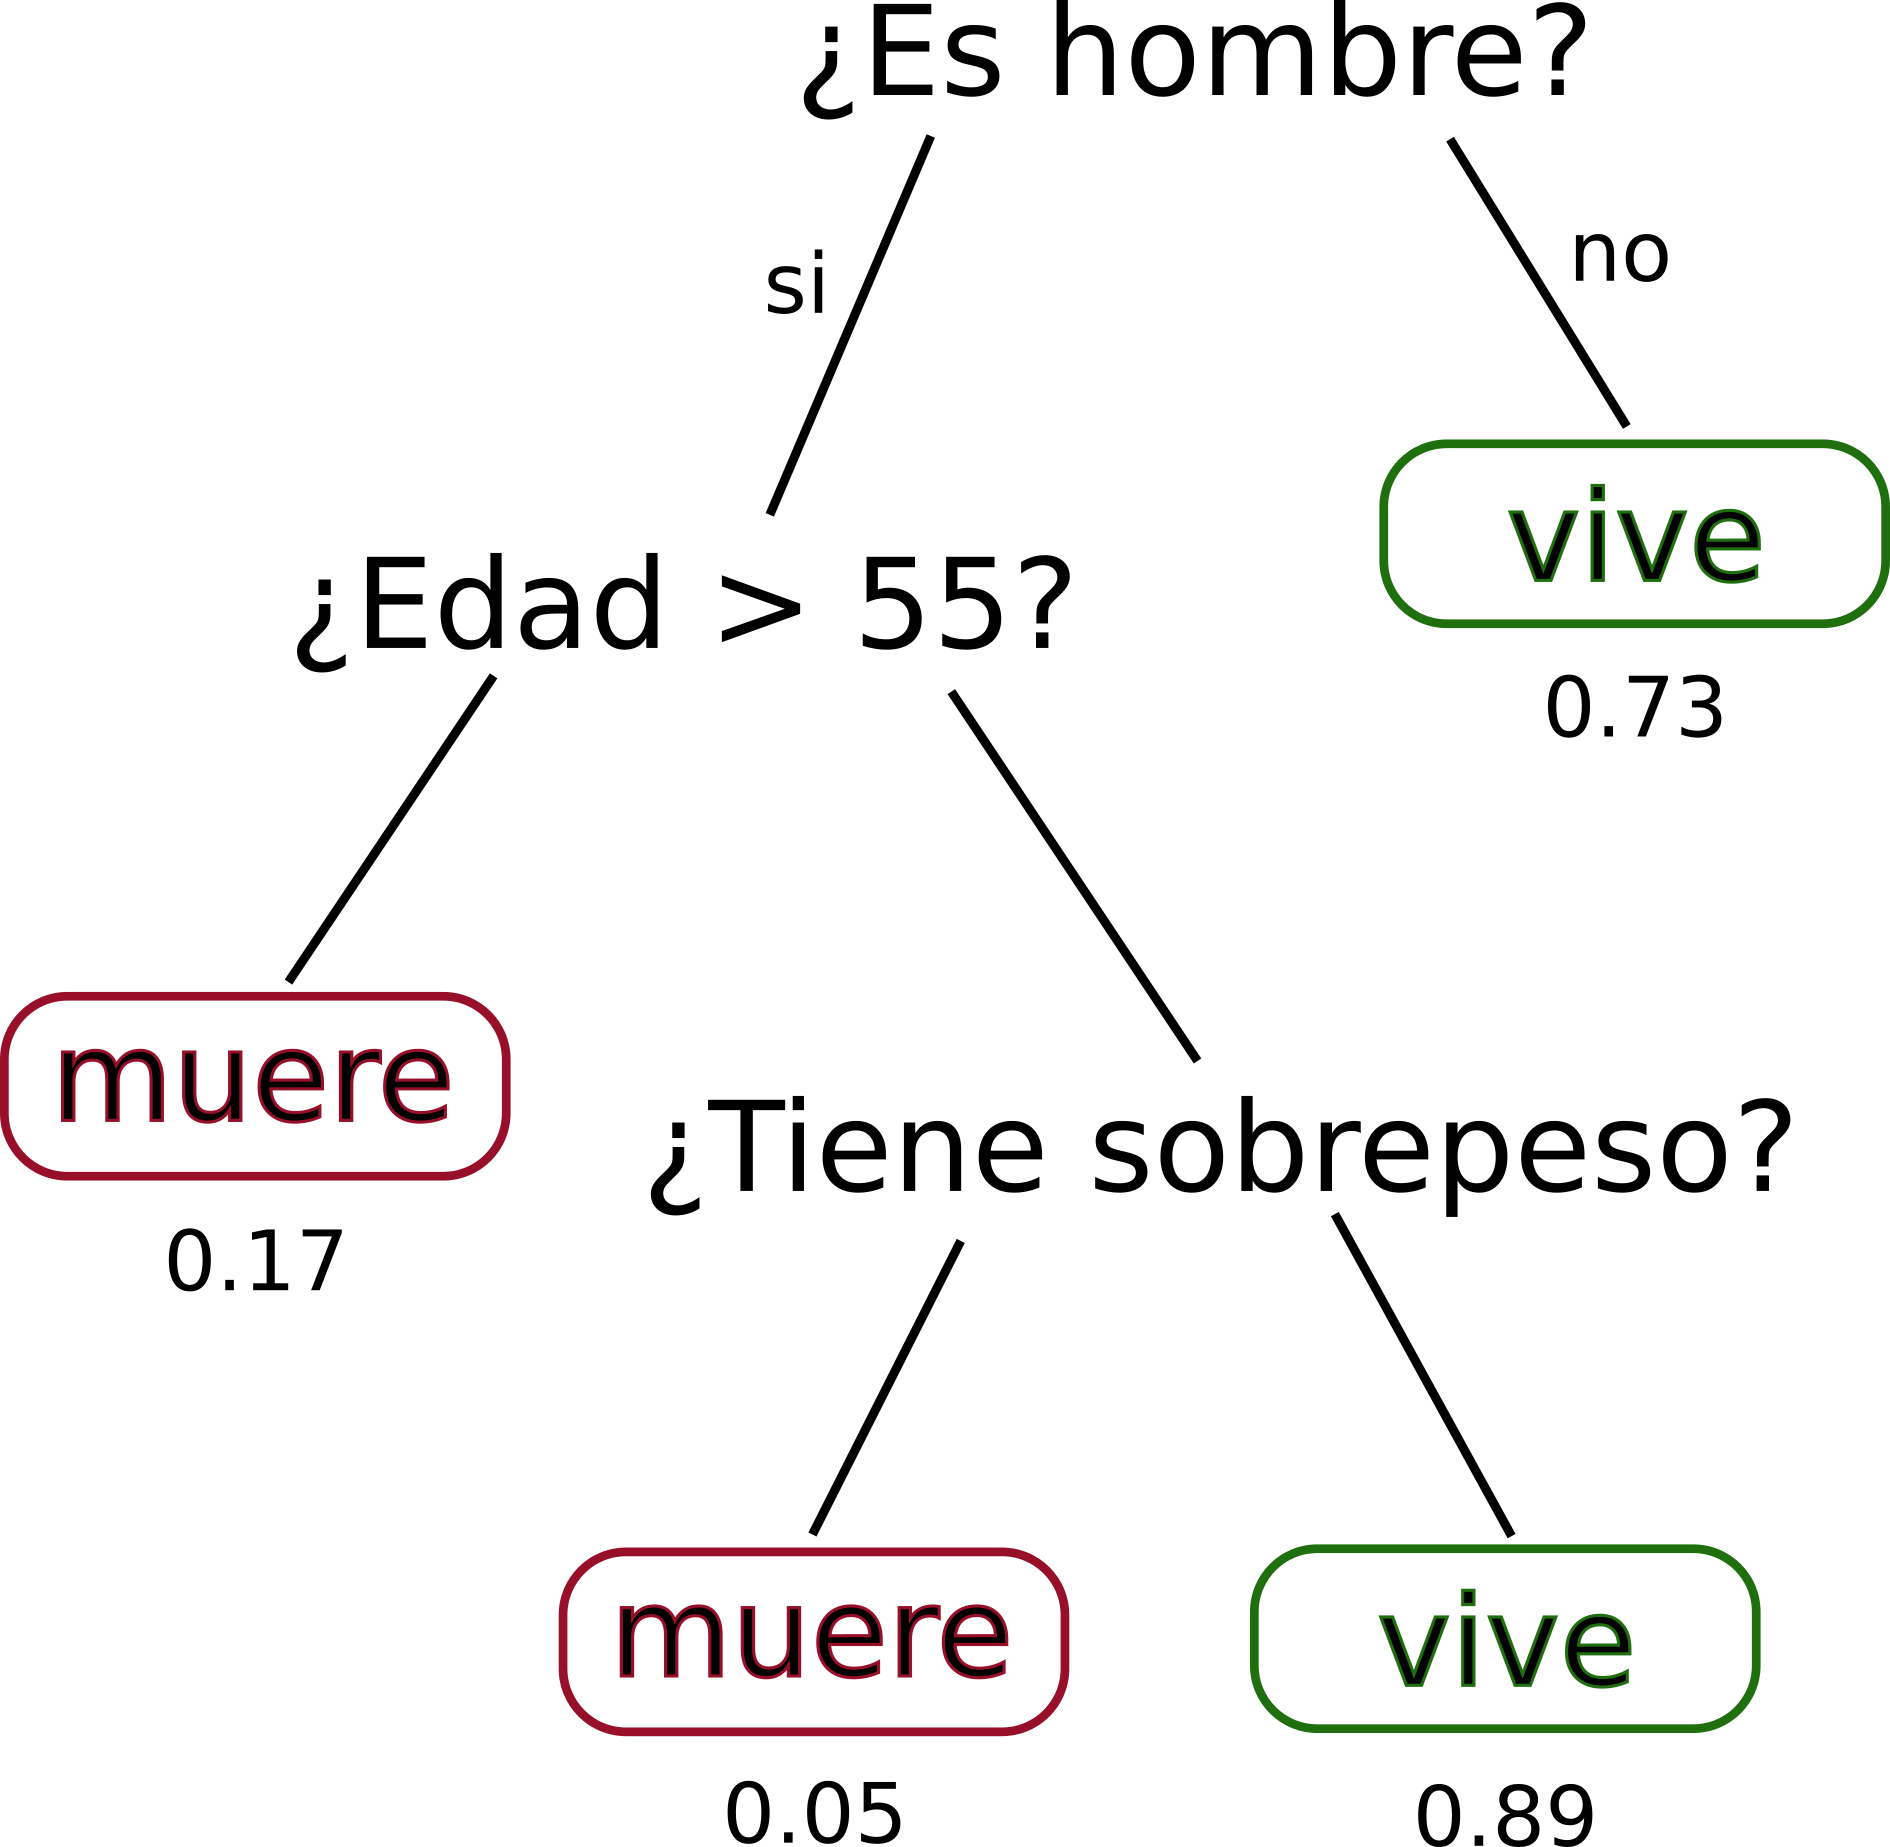
\includegraphics[width=0.4\linewidth]{graficos/propios/arbol_decision.png}
	\caption{Ejemplo de árbol de decisión}
	\label{fig:dt-eg}
\end{figure}

\section{Métodos de ensamble}

En el aprendizaje automático, los métodos de ensamble usan múltiples algoritmos de aprendizaje para obtener un mejor poder predictivo del que podría ser conseguido por cualquiera de los algoritmos constituyentes por sí solo.

Evaluar la predicción de un ensamble requiere más computaciones de las que requiere un modelo individual, así que los ensambles pueden ser imaginados como una manera para compensar algoritmos con un pobre aprendizaje realizando mucha computación adicional. Algoritmos rápidos como los árboles de decisión son comúnmente usados en los métodos de ensamble, sin embargo, otros algoritmos más lentos pueden beneficiarse de las técnicas de ensamble también.

\subsection{Random Forest}

\textit{Random Forest} es un método de construcción sistemática de un bosque de árboles de decisión. Se basa en un procedimiento pseudoaleatorio para seleccionar componentes de un vector de características, y los árboles de decisión son generados usando sólo los componentes seleccionados. Cada árbol generaliza la clasificación de nuevos puntos de diferentes maneras por las invarianzas de las características no seleccionadas. Las decisiones de los árboles son combinadas promediando las probabilidades en cada hoja \citep{ho1998random}.

Con \ac{RF} se obtienen importantes mejoras de exactitud respecto a un árbol de decisión entrenado con el conjunto de datos completo. Además, mientras que un bosque crece en complejidad (medida como el número de árboles) su exactitud en el conjunto de prueba no disminuye.

La figura \ref{fig:rf} ilustra el funcionamiento de \textit{Random Forest} de manera gráfica.

\begin{figure}[htbp]
	\centering
	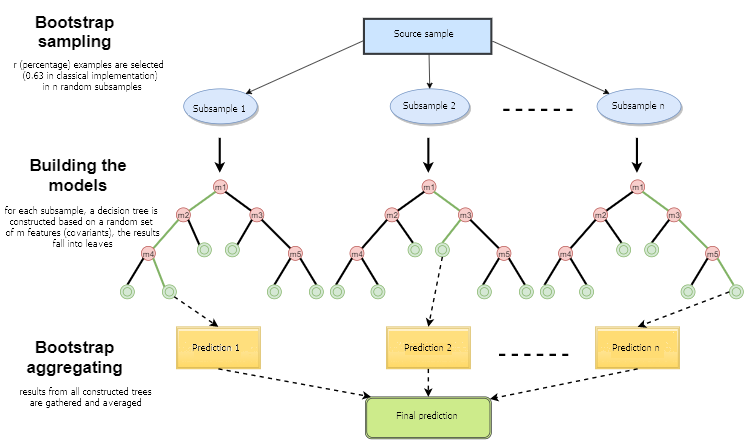
\includegraphics[width=\linewidth]{graficos/rf.png}
	\caption{Funcionamiento de Random Forest \citep{mql5:rf}}
	\label{fig:rf}
\end{figure}


\subsection{XGBoost}

\textit{Boosting} es un método similar a \textit{bagging} que agrupa varios modelos débiles en un modelo fuerte. La diferencia con \textit{bagging} es que no se crean muestras aleatorias con repetición, sino que se incrementa la exactitud del modelo de forma progresiva, haciendo que los módelos débiles se enfoquen más en las instancias mal clasificadas de los clasificadores anteriores. AdaBoost es un ejemplo simple de \textit{boosting} que se puede resumir en el los siguientes pasos:

\begin{enumerate}
	\item Se escoge una muestra aleatoria del conjunto de entrenamiento
	\item Se entrena un clasificador débil con esta muestra y se clasifica todo el conjunto de entrenamiento
	\item A las instancias mal clasificadas se les da más peso para que tengan más probabilidad de aparecer en la siguiente muestra
	\item Se repite este proceso de manera que las instancias mal clasificadas reciben un mayor enfoque de los clasificadores subsiguientes
\end{enumerate}

\textit{Gradient Boosting} por otro lado, modela el problema de clasificación como una función de pérdida que debe ser minimizada. Cada nuevo clasificador débil es un paso más en la dirección negativa de la gradiente, con lo que se minimiza el error. Está tecnica es susceptible de sufrir sobre ajuste.

Finalmente, XGBoost es una implementación de \textit{Gradient Boosting} en árboles de decisión creada por Tianqi Chen. La palaba extreme se refiere a la meta de ingeniería de aprovechar los recursos computacionales al límite, lo que provocó que su uso se expandiera rápidamente en la comunidad.

% \section{Recomendaciones generales de escritura}
% Un trabajo de esta naturaleza debe tener en consideración varios aspectos generales:

% \begin{itemize}
% \item Ir de lo genérico a lo específico. Siempre hay qeu considerar que el lector podría ser alguien no muy familiar con el tema
% y la lectura debe serle atractiva.
% \item No poner frases muy largas. Si las frases son de mas de 2 líneas continuas es probable que la lectura sea dificultosa.
% \item Las figuras, ecuaciones, tablas deben ser citados y explicados {\bf antes} de que aparezcan en el documento.
% \item Encadenar las ideas. Ninguna frase debe estar suelta. Siempre que terminas un párrafo y hay otro a continuación,
% el primero debe dejar abierta la idea que se explicará a continuación. Todo debe tener secuencia.
% \end{itemize}

\subsection{Método de ensamble para datos desbalanceados}


Muchos algoritmos de clasificación han demostrado un desempeño no óptimo en problemas con clases desbalanceadas \citep{batista2004study, mani2003knn, seiffert2010rusboost}.

El \textit{bagging} es un método de aprendizaje de ensamble que podría resolver este problema si los clasificadores base fueran certeros y diversos \citep{breiman1996bagging}. Sin embargo, cada clasificador base dentro del \textit{bagging} aún sufre del mismo problema, puesto que las instancias se muestrean proporcionalmente del conjunto original. Incluso si se balancean los datos antes de ejecutar los algoritmos de aprendizaje, se altera la distribución original y se hace overfitting.

El método de \textit{bagging} propuesto \citep{sun2015novel} ataca un problema desbalanceado convirtiéndolo en varios problemas balanceados, lo cual incluye tres componentes: \textit{Balanceo del conjunto de datos, Modelamiento y Clasificación}. La figura \ref{fig:bagging-imbalanced} muestra los detalles.

\begin{figure}[htbp]
	\centering
	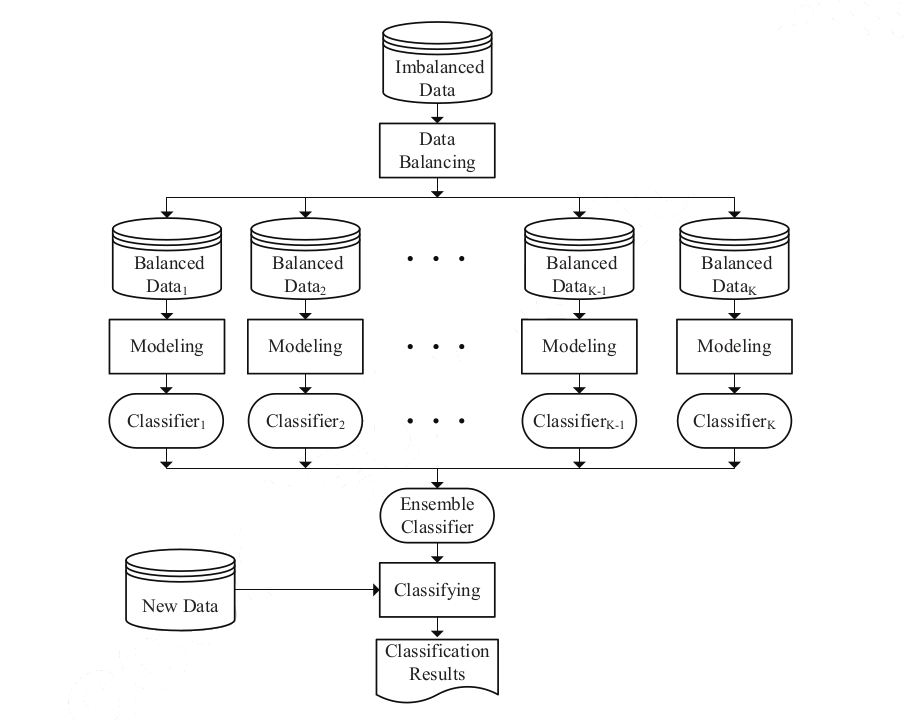
\includegraphics[width=\linewidth]{graficos/bagging_imbalanced.png}
	\caption{Método de \textit{bagging} propuesto \citep{sun2015novel}}
	\label{fig:bagging-imbalanced}
\end{figure}

En este método, la clase mayoritaria genera varios subsets mediante muestreo sin repetición. Cada subset tiene un número de instancias igual a la clase minoritaria, y luego se combinan con esta. Así, se obtienen varios conjuntos de datos balanceados (Balanceo de los datos). Luego, cada conjunto se usa para crear un clasificador binario con un algoritmo específico (Modelamiento). Finalmente estos clasificadores binarios se combinan en un ensamble para clasificar nuevas instancias (Clasificación).

Esta combinación de los resultados de los clasificadores base se realiza mediante un promedio ponderado por la inversa de la distancia de la instancia a clasificar con el subset utilizado. De esta manera, los subsets más parecidos a la nueva instancia tendrán un mayor peso en la decisión final.


\section{Evaluación de los modelos}

\subsection{Exactitud, Precisión y Exhaustividad}

De forma intuitiva se pueden definir de la siguiente manera:

\begin{description}
	\item [Exactitud] Porcentaje de clasificaciones correctas. En inglés: \textit{accuracy}.
	\item [Precisión] De aquellos clasificados como positivos, cuántos son realmente positivos. En inglés: \textit{precision}.
	\item [Exhaustividad] De los realmente positivos, cuántos fueron clasificados como tal. En inglés: \textit{recall}.
\end{description}

Por otro lado, para definir estos térmios rigurosamente, es necesario explicar la matriz de confusión, también conocida como tabla de contingencia. Esta es una herramienta que permite visualizar el desempeño de un algoritmo de clasificación. Contrasta las clasificaciones hechas con la clase verdadera. Los números en la diagonal representan el error o confusión entre las clases \citep{fawcett2006introduction}.

En la figura \ref{fig:confussion2} se muestra una matriz de confusión con 2 clases.

\begin{figure}[htbp]
	\centering
	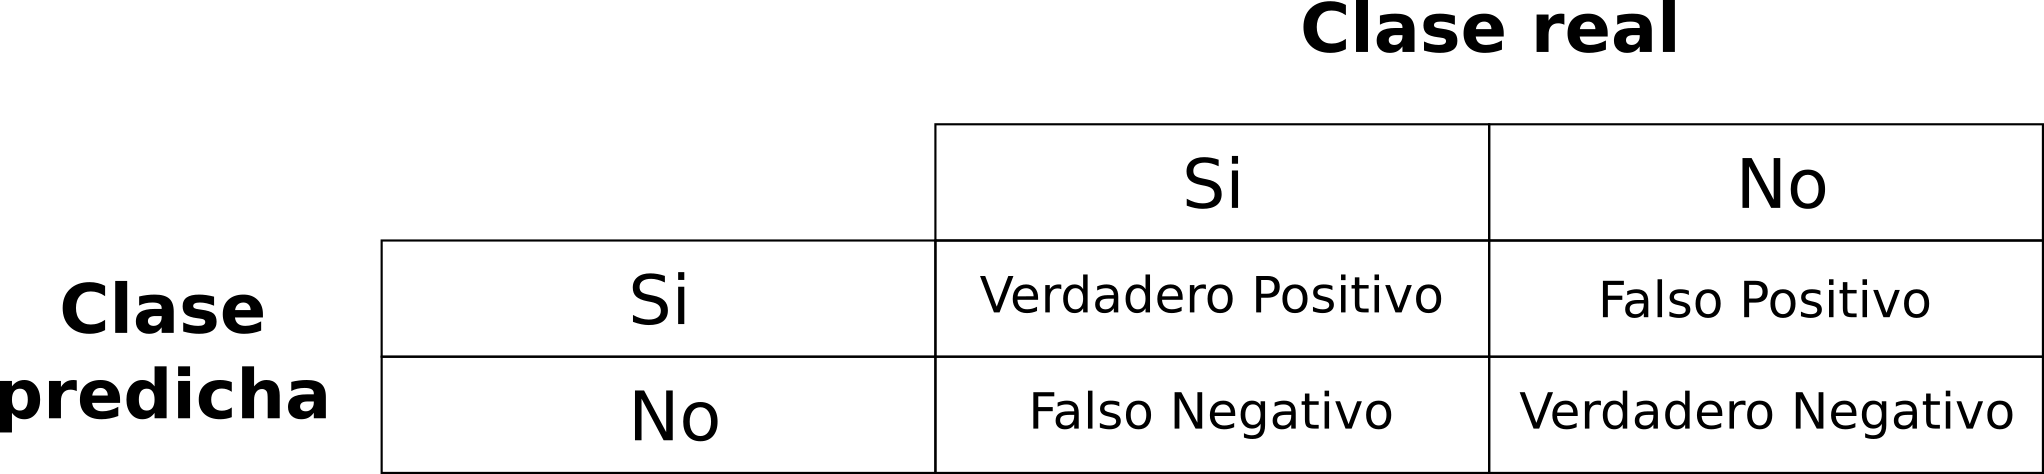
\includegraphics[width=0.6\linewidth]{graficos/propios/matriz_confusion.png}
	\caption{Matriz de confusión de dos clases}
	\label{fig:confussion2}
\end{figure}

A partir de esta matriz se pueden definir formalmente la exactitud, precisión y exhaustividad. Esta definición es presentada en la fórmula \ref{eq:accuracy-prec-rec}.

\begin{equation}
	\label{eq:accuracy-prec-rec}
\begin{split}
	\text{Exactitud} &= \frac{\text{verdaderos positivos} + \text{verdaderos negativos}}{\text{verdaderos positivos} + \text{falsos positivos} + \text{verdaderos negativos} + \text{falsos negativos}} \\\\
	\text{Precisión} &= \frac{\text{verdaderos positivos}}{\text{verdaderos positivos} + \text{falsos positivos}} \\\\
	\text{Exhaustividad} &= \frac{\text{verdaderos positivos}}{\text{verdaderos positivos} + \text{falsos negativos}}
\end{split}
\end{equation}

Para utilizar los diferentes modelos, hay que definir una etiqueta positiva y una etiqueta negativa. Normalmente, la etiqueta positiva se destina a las créditos morosos. Sin embargo, si se invierte esta etiqueta y se hace que los créditos morosos tengan la etiqueta negativa, entonces la precisión y la exhaustividad se pueden asociar con conceptos mucho más intuitivos:

\begin{description}
	\item [Precisión] De las personas que el modelo clasificó como buenos pagadores, cuántos realmente pagan sus préstamos. En otras palabras esta métrica se convierte en $1 - \text{\% de morosidad}$. Y representa muy bien el riesgo crediticio del modelo.
	\item [Exhaustividad] Del universo de buenos pagadores, cuántos pueden ser capturados con este modelo. Está métrica tiene una incidencia directa en el costo de adquisión de los clientes.
\end{description}

En otras palabras, el balance entre precisión y exhaustividad se convierte en el balance entre el riesgo que se quiere asumir y el costo de adquisición de los clientes y el tamaño del mercado. En cambio el concepto de Exactitud no tiene una incidencia directa en algún aspecto del problema, además de que no es una buena métrica a utilizar en conjuntos desbalanceados.

Pongamos un ejemplo extremo de desbalance, donde sólo una persona de cada 1000 no paga su crédito. Un modelo que simplemente trate de maximizar la exactitud puede aprender erróneamente a clasificar a todos como si pertenecieran a la clase mayoritaria, obteniendo así una exactitud de 0.999.

En estos casos de desbalance tan extremo también la precision y la exhaustividad se ven afectadas, cosa que se soluciona invirtiendo las clases, i.e. haciendo que 0 sean las personas que pagan y 1 las personas que no pagan adecuadamente. Con esta disposición, y con el mismo ejemplo de tener 1 moroso en 1000 personas, la precisión sería de 0 y la exhaustividad también, indicando que nuestro modelo no tiene poder predictivo.

\subsection{Curva ROC y Area bajo la curva (AUC)}

Las métricas vistas en la sección anterior tienen un inconveniente: es necesario encontrar un punto de corte para poder calcularlas. La curva ROC en cambio, evalúa y compara el desempeño de los algoritmos sin necesidad de escoger un punto de corte.

La curva ROC grafica la relación entre la razón de verdaderos positivos y la razón de falsos positivos según se varía el umbral de discriminación. Mientras esta curva se acerque más a la esquina superior izquiera, mejor será la clasificación.

El \ac{AUC} es una medida que nos permite comparar diferentes curvas fácilmente. Funciona calculando el área debajo de la curva ROC, tal como su nombre lo indica. Ver figura \ref{fig:eg-roc}.

\begin{figure}[htbp]
	\centering
	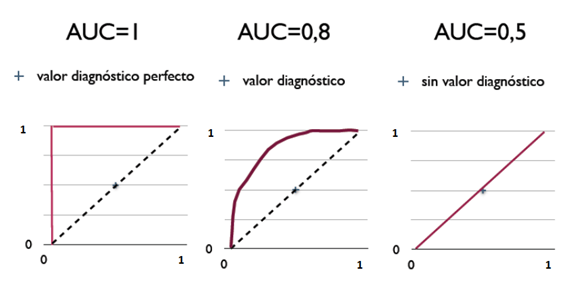
\includegraphics[width=0.8\linewidth]{graficos/eg_roc.png}
	\caption{Ejemplo de curvas ROC \citep{wiki:roc_figure}}
	\label{fig:eg-roc}
\end{figure}

Finalmente cabe mencionar que pueden existir dos curvas ROC diferentes que tengan la misma área bajo la curva. Por eso no se puede descartar el uso de las curvas ROC totalmente, ya que dependiendo de a qué se le quiera dar más importancia, se escogerá una curva y otra. Tarea que es imposible solamente observando el \ac{AUC}.

%\section{Repeated-N cross fold validation}


%\section{Pruebas de hipótesis estadísticas}

%\subsection{Pairwise comparison}
%\subsection{Analysis of variance}
%\subsection{Friedman test}
%\subsection{Friedman test with post-hoc test}
%Demšar, J. (2006). Statistical comparisons of classifiers over multiple data sets. Journal of Machine Learning
%Research, 7, 1-30.
%\subsection{Press Q statistic}

\section{Trabajo relacionado}

Desde que se creó la calificación crediticia en 1956, se han investigado diferentes métodos para mejorar el poder predictivo de los modelos utilizados. A continuación se hará un breve resumen de algunas investigaciones recientes.

En \citep{sohn2016technology} se propone una regresión logística difusa para explotar mejor atributos de evaluación linguísticos. Los resultados son que efectivamente se mejora el desempeño respecto a una regresión logística normal. En \citep{bahnsen2014example} se propone una regresión logística que usa una matriz de costo dependiendo de cada ejemplo. Los resultados subrayan la importancia de usar los costos financieros reales, ya que se logran mejoras significativas en términos de ahorro de dinero.

Por otro lado en \citep{zhao2015investigation} se aplica una \ac{MLP} que se trata de optimizar mediante (i) la mejora de la distribución de los datos usando un método llamado Average Random Choosing, (ii) probando diferentes tamaños de conjuntos de train-test-validation y (iii) encontrar el número óptimo de neuronas ocultas. Los resultados son bastante alentadores y los autores claman que se pueden utilizar incluso fuera del dominio de los puntajes de crédito.

En el área de aprendizaje profundo también se ha hecho progreso. Particularmente en \citep{luo2017deep} se hace uso de una \ac{DBN} que se compara con algoritmos más populares de calificación crediticia como \ac{LR}, \ac{MLP} y \ac{SVM}. Los modelos son aplicados en un conjunto de contratos CDS XR 14 (sin reestructuración) y los resultados arrojan que la \ac{DBN} tiene la mejor exactitud y AUC.

En \citep{huang2007credit} se usan tres estrategias para construir modelos híbridos de \ac{SVM}, las pruebas se ejecutan con dos conjuntos de datos crediticios de la UCI. Comparados con redes neuronales, programación genética y clasificadores de árboles, los \ac{SVM} tienen una exactitud idéntica con relativamente pocas características. Adicionalmente, al combinar algoritmos genéticos con \ac{SVM}, se puede realizar simultáneamente la selección de variables y la optimización de parámetros del modelo.

En otro estudio \citep{harris2015credit} se introduce el uso de \ac{CSVM} para calificación crediticia. Este algoritmo resolvería algunas limitaciones \ac{SVM}, particularmente se centra en el costo computacional en conjuntos grandes, logrando niveles de clasificación similares mientras se mantiene un costo computacional bajo.

En \citep{malekipirbazari2015risk} se propone una clasificación basada en \ac{RF}. Se utilizan los datos de préstamos peer2peer Lending Club, y los resultados indican que los métodos basado en \ac{RF} superan los score crediticios del FICO así como los propios scores de LC.

Además se presentan algunos métodos nuevos, como el \ac{RF} paralelo de \citep{van2016novel}. Donde al integrar el modelo en el proceso de selección de variables se mejora la exactitud promedio obteniendo un 76.2\%.

En \citep{xia2017boosted} y \citep{bhatia2017credit} se experimenta con \ac{XGBoost}. En el primer artículo se centra en el ajuste de los parámetros del modelo, mientras que el segundo hace una comparación más amplia con otros modelos como \ac{LDA} y \ac{RF}.

Los préstamos \ac{P2P} son una opción para tomar préstamos de personas individuales sin utilizar un banco o una entidad financiera tradicional. En \citep{zhang2016research} se usa un conjunto de datos \ac{P2P} para construir un modelo basado en árboles de decisión fusionando datos de los medios de comunicación sociales. En \citep{zang2014credit} también se usa un conjunto de datos \ac{P2P}, perteneciente a Lending Club. Se aplica una \ac{MLP} y se obtienen resultados favorables. Para terminar con \ac{P2P}, en \citep{tan2018deep} se utiliza una red neuronal profunda para modelar los riesgos en competencia, el del prestamista y el del prestatario, este sería el primer lugar donde se prueba dicho concepto obteniendo un desempeño interesante en las inversiones.

En \citep{nanni2009experimental} se prueban varios clasificadores de ensamble en los datos de crédito Alemán y Australiano. Dichos clasificadores ensamblados mejoran el desempeño de sus respectivos clasificadores base. En \citep{brown2012experimental} se hace un estudio comparativo de varios modelos en cinco conjuntos de datos distintos. Se hace un énfasis especial en el desbalanceo de la datos, pues se hace un undersampling de la clase minoritaria para pronunciar el desbalance cada vez más y evaluar como se van comportando los modelos en cada caso. Los resultados son que \ac{RF} y clasificadores de \textit{Gradient Boosting} se desempeñan bien incluso en conjuntos de datos altamente desbalanceados. Finalmente en \citep{wang2012two} se proponen dos estrategias de ensamble para árboles, que luego se comparan con cinco clasificadores base y cuatro clasificadores de ensamble, obteniendo resultados competitivos.

En conclusión, hasta la fecha se ha venido realizando un trabajo muy diverso. El área de calificación crediticia es un área muy fértil, pero aún quedan muchas potenciales mejoras por realizarse.

\section{Consideraciones Finales}

Ahora que tenemos una idea clara de cómo funcionan los clasificadores base, los ensambles y los métodos de evaluación; podemos pasar a explicar los conjuntos de datos utilizados, la metodología y los experimentos realizados.
